% Nejprve uvedeme tridu dokumentu s volbami
\documentclass[czech,master,public,dept460,male,cpdeclaration]{diploma}	% jednostranny dokument

\usepackage[utf8]{inputenc}
\inputencoding{utf8}
\usepackage[czech]{babel}

\usepackage{subfig}		% makra pro "podobrazky" a "podtabulky"
\usepackage{tikz}		% makra pro kresleni

\usepackage{makecell}

\usepackage{pdflscape}

\usepackage{placeins}


\newcommand{\iic}{I\textsuperscript{2}C }
\newcommand{\iis}{I\textsuperscript{2}S }
\newcommand{\eeprom}{E\textsuperscript{2}PROM}

\newcommand{\VID}{0x04D8}
\newcommand{\PID}{0xF32C}

%\widowpenalty10000
%\clubpenalty10000


% Zadame pozadovane vstupy pro generovani titulnich stran.
\ThesisAuthor{Bc. Pavel Kovář}

% U bakalarske praxe neni nutne nazev zadavat
\CzechThesisTitle{Modul USB FM rádia}

% U bakalarske praxe neni nutne anglicky nazev zadavat
\EnglishThesisTitle{USB FM Radio Modul}

\SubmissionDate{29. dubna 2016}

%\PrintPublicationAgreement{true}

\Thanks{Rád bych na tomto místě poděkoval mému vedoucímu panu Ing. Davidu Seidlovi, Ph.D. za cenné rady a trpělivost.}

\CzechAbstract{Tato práce popisuje návrh USB FM přijímače se dvěma tunery. Jeden tuner slouží pro přehrávání zvuku a~druhý pro vyhledávání dalších stanic. Přijímač je v~systému reprezentován jako USB zvuková karta.\\ 
Příjem je realizován dvojicí integrovaných obvodů Si4735-DU. Tyto jsou přes \iis a \iic  spojeny s~MCU PIC32MX250F128B, který přes USB zajišťuje komunikaci s počítačem. V rámci firmware MCU je, po neúspěchu s Microchip harmony frameworkem, napsán vlastní USB stack.\\
Knihovna je napsána v jazyku~C s~využitím knihovny libusb. Poskytuje funkce pro tři úrovně přístupu k~tunerům.\\
Demonstrační aplikace je ve formě grafického uživatelského rozhraní, napsaná  v~C++ s využitím QT frameworku.\\
Vše je funkční pod OS Linux i~Windows.}

\CzechKeywords{FM rádio, USB, RDS, QT, libusb, PIC}

\EnglishAbstract{This work describes design of USB FM radio receiver with two tuners. One tuner is for radio playback, second one seeks new stations. In computer, device acts as sound card.\\
Receiving is done by couple of Si4735-DU integrated circuits, which are connected to MCU via \iic and \iis. MCU forwards data over USB to computer and back. Use of Microchip harmony framework was not successful so in firmware is USB stack written from scratch.\\
Library is written in C with use of libusb library. There are three levels of functions to access tuners.\\
Demo application has graphical user interface and is written in C++ in QT framework.\\
All works under Linux and Windows.}

\EnglishKeywords{FM radio receiver, USB, RDS, QT, libusb, PIC}

% Pridame pouzivane zkratky (pokud nejake pouzivame).
\AddAcronym{AM}{Amlitudová Modulace (Rozhlasové vysílání v pásmu dlouhých vln)}
\AddAcronym{CD}{Compact disc}
\AddAcronym{DAB}{Digital Audio Broadcasting (Digitální pozemní rozhlasové vysílání)}
\AddAcronym{DIP}{Dual Inline Package}
\AddAcronym{FM}{Rozhlasové vysílání v pásmu velmi krátkých vln}
\AddAcronym{HTML}{Hypertext Markup Language}
\AddAcronym{\iic}{Inter-Integrated Circuit}
\AddAcronym{\iis}{Integrated Interchip Sound}
\AddAcronym{LW}{Long Waves (Rozhlasové vysílání v pásmu dlouhých vln)}
\AddAcronym{MCU}{Microcontroller unit}
\AddAcronym{OS}{Operační systém}
\AddAcronym{PCM}{Pulse-code modulation}
\AddAcronym{RDS}{Radio Data System}
\AddAcronym{SPI}{Serial Peripheral Interface}
\AddAcronym{SSOP}{Shrink Small-Outline Package}
\AddAcronym{SW}{Short Waves (Rozhlasové vysílání v pásmu krátkých vln)}
\AddAcronym{USB}{Universal Serial Bus}
\AddAcronym{UTF-16}{Způsob kódování znaků ISO 10646/Unicode}
\AddAcronym{QFN}{Quad Flat No-leads package}



% Zadame cestu a jmeno souboru ci nekolika souboru s digitalizovanou podobou zadani prace
% Pri sazbe se pak hledaji soubory Figures/Zadani1.jpg, Figures/Zadani2.jpg atd.
% Do diplomove prace se postupne vlozi vsechny existujici soubory Figures/ZadaniXXX.jpg
% Pokud toto makro zapoznamkujeme sazi se stranka s upozornenim
\ThesisAssignmentImagePath{figures/zadani}

% Zadame soubor s digitalizovanou podobou prohlaseni
% Pokud toto makro zapoznamkujeme sazi se cisty text prohlaseni
%\DeclarationImageFile{figures/Prohlaseni.jpg}



% Zacatek dokumentu
\begin{document}

% Nechame vysazet titulni strany.
\MakeTitlePages


\section{Úvod}
\label{sec:Uvod}
%Tento text je ukázkou sazby diplomové práce v \LaTeX{}u pomocí třídy dokumentů \verb|diploma|.

Cílem této diplomové práce je navrhnout USB FM přijímač rádiového vysílání. Přijímač bude v systému reprezentován jako zvuková karta a bude obsahovat dva tunery. Jeden bude sloužit k samotnému příjmu vysílání a druhý k vyhledávání dalších stanic. Dále napsat knihovnu, umožňující ovládání tuneru pod Operačními systémy Linux a Windows. Text této práce je členěn do třech kapitol.

První kapitola se zabývá konstrukcí modulu. Je zde shrnuto a~zhodnoceno několik možností jak realizovat jednak samotný příjem rozhlasového vysílání a~také několik možností řešení napojení tunerů na USB sběrnici.

Druhá kapitola je věnována popisu vybraného tuneru. Je zde uveden zvolený způsob získání zvukových dat, filozofie ovládání tuneru a popis všech použitých příkazů pro tuneru.

Ve třetí kapitole je rozebráno napojení tunerů na USB sběrnici. Je zde pois USB popis porblémů s harmony , chyby v křemíku použitého MCU, porblémy nesynchronizovaných hodin udesílání zvuku. Popsáno vzniklé USB rozhraní (TODO)

Čtvrtá kapitola se věnuje vzniklé knihovně a demonstračnímu programu. V první části kapitoly je popis filozofie a rozvrstvení knihovny včetně popisu funkcí. Doplněno ukázkovým kódem práce. Závěru kapitoly je popsána demonstrační aplikace. (TODO)

%V závěru jsou shrnuty dosažené cíle, vyzdvihnut vlastní přínos

\section{Výběr součástek}
\label{sec:Vyber}
Vzhledem k tomu, že není možné se cenou zařízení přiblížit zavedeným výrobcům elektroniky, rozhodl jsme se výběr součástek a konstrukci modulu přizpůsobit tak, aby bylo možné modul vyrobit v domácích podmínkách.

%mužeš přidat zmínku o snaze mít možnost rozšiřování funkcionality po strance FW a SW
 
\subsection{Volba rozhraní pro spojení modulu a počítače}
Po tomto rozhraní se budou přenášet dva druhy informací a to samotný zvuk a ovládání tunerů.\\
V současné době je prakticky jediným schůdným řešením použití rozhraní USB díky celé řadě výhod, které nabízí. Zejména jeho širokým rozšířením na téměř všech počítačích, od osobních přes servery až po jednodeskové či průmyslové počítače. Stejně tak je k dispozici velké množství součástek se zabudovanou podporou tohoto rozhraní. USB dále poskytuje možnost napájení připojených zařízení až do příkonu 2,5W. Má zabudovanou podporu pro různé druhy přenosů včetně isochronních (garantovaný periodický přenos předem dohodnutého množství dat). Specifikace USB zavádí standardní třídy funkcí v zařízení. V době psaní tohoto textu sice neexistuje třída pro ovládání tuneru, ale existuje třída popisující zvuková zařízení. Díky tomuto není potřeba vyvíjet vlastní ovladač zvukové karty na straně počítače.\\
%mužeš to vycpat textem o PCI - PCI-e

-je nemožné konkurovat cenou
-hoby platforma
-způsoby jak to vyřešit 
 -diskrítní tuner
 -analogový zvuk
 -digitální zvuk
-připojení s PC USB
- požadavky na USB


Bud v uvodu a nebo tady zmínit, že pro nemožnost konkurovat výrobcům spotřební elektroniy byl výběr součástek a celá konstrukce přispůsobena možnosti amatérké výroby a dostupnosti součástek u nás.

\subsection{Způsob příjmu rozhlasového vyslání}
Jednou možností je řešení příjmu z diskrétních součástek a nebo s pomocí analogových IO. Ovšem toto je příliš komplikované.\\
Na trhu je ovšem řada integrovaných obvodů, které zajišťují samotný příjem vysílání včetně vyhledávání static, měření kvality signálu a přijmu RDS a to s minimem potřebných externích součástek. Tyto IO se typicky ovládají pomocí \iic nebo SPI a zvuk poskytují digitálně přes rozhraní \iis a nebo analogově.\\
Bohužel drtivá většina je dostupná pouze v pouzdru QFN, které se velmi obtížně pájí a v minimální množství 1000 kusů. Výjimkou je SI4735-D60 od výrobce SILICON LABS, který je dostupný v pouzdru SSOP24 a je možné jej u nás zakoupit i po jednotlivých kusech. IO neumožňuje přijímat DAB, ale umí nasledující:
\begin{itemize}
\item{Pásma: FM, SW, MW, LW}
\item{Vzorkovací frekvence až do 48kHz}
\item{Rozlišení vzorku kanálu až do 24bitů}
\item{Stereofonní příjem.}
\item{Příjem RDS}
\end{itemize}


\subsection{I2S -> USB}
	TAS x Osmi bit x PIC32mx

\section{Tuner}
\label{sec:tuner}


\subsection{I2S}
	Popis\\
	Problém synchronizace hodin
	
	
\subsection{Ovládání tuneru}
\subsubsection{RDS}
		čtení z tuneru\\
		dekódování základních informací

\section{USB}
\label{sec:USB}
Na rozdíl od například populárního rozhraní UART je USB podstatně komplikovanější. Je to určitou daní za jeho univerzálnost. Vzhledem k velkému rozsahu specifikace USB \cite{usb-spec} se omezím pouze na popis částí nezbytných pro implementaci modulu.\\
S vydáním specifikace USB 2.0 byly předchozí specifikace označeny jako zastaralé a neměly by se používat pro nové konstrukce. Následující text se tedy týká USB 2.0 a~rychlosti full-speed.

%minimální zařízení\\


\subsection{Stručný úvod do full-speed USB 2.0}
\subsubsection{Topologie}
\InsertFigure{figures/usb-functions.eps}{100mm}{USB endpointy a funkce.}{fig:usb-functions}

TODO Obrázek s pyramidou topologie

%TODO obrázek topologie \InsertFigure{figures/usb-functions.eps}{100mm}{USB endpointy a funkce.}{fig:usb-topo}
Ačkoliv název rozhraní (Univerzální Sériová Sběrnice) napovídá, že jde o sběrnici, jedná se o zapojení typu hvězda. Přesněji, jak je vidět z obrázku \ref{fig:usb-topo}, připojená zařízení a rozbočovače tvoří strom jehož kořenem je hostitel. Tento implementuje tzv. kořenový rozbočovač (root hub), ke kterému je možné buď přímo připojit jedno zařízení a nebo rozbočovač a do něj dalších až osm zařízení/rozbočovačů. Je možné takto za sebe zřetězit až pět rozbočovačů. Celkově je možné na jeden kořenový rozbočovač připojit až 127 zařízení (včetně rozbočovačů).\\
Velkou výhodou je, že zařízení je od topologie odstíněno. Vždy se z jeho pohledu komunikuje přímo s hostem.\\
Ve specifikaci je také zohledněn fakt, že zařízení zpravidla nezastává pouze jedinou funkci. To je konec konců případ i tohoto modulu. Obsahuje dvě funkce - zvukovou kartu a \iic tunel pro komunikaci s tunery.

\subsubsection{Komunikace}

\begin{table}[!ht]
\begin{center}
\begin{tabular}{|l|c|c|c|c|}
\hline 
 & Latence & \makecell{Vyhrazená šířka\\ pásma} & \makecell{Spolehlivý\\ přenos} & Typ dat \\ 
\hline 
Isochroní přenos & Minimální & až 90\% & Ne & Proud \\ 
\hline 
Hromadný přenos & Negarantovaná & Ne & Ano & Proud \\ 
\hline 
Přenos přerušení & Minimální & až 90\% & Ano & Proud \\ 
\hline 
Řídící přenos & Negarantovaná & až 10\% & Ano & Zprávy \\ 
\hline 
\end{tabular} 
\end{center}
\caption{Druhy USB přenosů.}
\label{tab:usb-transfer-types} 
\end{table}

Aby bylo možné uspokojit nároky na přenos (transfer) dat rozdílné povahy různými funkcemi, zavádí specifikace koncové body (endpoint). Osm výstupních (OUT) pro směr z hostitele do zařízení a osm pro směr opačný (IN). Směr je vždy určován právě z pohledu hostitele. Každému bodu je možné přiřadit jeden ze čtyř druhů přenosu podle tabulky \ref{tab:usb-transfer-types}. Výjimkou je  vstupní a výstupní koncový bod nula. Tyto vždy slouží pro řídící přenosy a na rozdíl od ostatních bodů je musí podporovat všechna zařízení.
Full-speed USB podporuje čtyři druhy komunikace uvedené v tabulce \ref{tab:usb-transfer-types}.\\ 
Body nula jsou využívány jednak k inicializaci a správě vlastního zařízení, ale také můžou být využívány zároveň i funkcemi. Například popisovaný modul jej využívá pro ovládání audio funkce.
Modul dále využívá vstupní koncový bod 1 pro přenos zvuku do hostitele a potom dvojici koncových bodů 2 v obou směrech pro komunikaci s tunery viz. obrázek \ref{fig:usb-functions}.\\
Přenos vždy sestává z alespoň jedné transakce (transaction), která se dále dělí na pakety (packets). Transakce je z pohledu zařízení vždy vyřizována od počátku do konce bez přerušení jinou transakcí. Je vždy iniciována vysláním token paketu hostitelem, který takto může řídit šířku pásma přidělovanou jednotlivým zařízením na sběrnici. Token pakety mohou být podle druhu transakce následujících třech druhů:
\begin{itemize}
\item \textbf{IN} (Vstupní) - Následuje přenos ze zařízení do hostitele.
\item \textbf{OUT} (Výstupní) - Následuje přenos z hostitele do zařízení.
\item \textbf{SETUP} - Následuje řídící přenos. %TODO ověř i a doplň překlad
\end{itemize}
Za tímto paketem následuje nula nebo více paketů s daty. Aby bylo možné detekovat výpadek nebo duplikaci některého z~paketů jsou specifikovány hned dva typy paketů. A~to DATA0 a~DATA1. U izochronních transakcí se vždy posílají pakety DATA0. U ostatních transakcí se vyšle nejprve DATA0 a~poté se~tyto druhy paketů střídají nezávisle na transakcích. Znovu se~od~DATA0 začne pouze v~následujících případech:
\begin{itemize}
\item Na začátku každé řídící transakce.
\item Po následujících žádostech hostitele (bude popsáno dále):
\begin{itemize}
\item Přiřazení konfigurace.
\item Zrušení zastavení koncového bodu.
\item Nastavení rozhraní.
\end{itemize}
\end{itemize}
Za datovými pakety následuje potvrzování transakce protistranou. Izochronní přenosy potvrzování nepodporují, tudíž datovými pakety jejich transakce končí. Transkace hromadných přenosů a přenosu přerušení jsou vždy zakončeny jedním potvrzovacím (handshake) paketem.  Transkace řídících přenosů mají před potvrzovací paket vložen jeden datový paket nulové délky (zero length packet často zkracovaný ZLP), ale opačného směru než všechny předchozí datové pakety. Potvrzovací paket vždy vysílá zařízení. Má vždy jeden z následujících typů:
\begin{itemize}
\item \textbf{ACK} (Úspěch) - Úspěšné ukončení transakce.
\item \textbf{NAK} (Neúspěch) - Typicky poškozená přijímaná data a nebo častěji zařízení nemá připravena data k odeslání.
\item \textbf{STALL} (Chyba) - Zařízení takto reaguje na požadavek, který nepodporuje.
\end{itemize}
Rozdíl mezi NAK a STALL je, že po NAK potvrzení bude hostitel požadavek opakovat (počet opakování není explicitně specifikován), kdežto STALL signalizuje nemožnost vyřízení požadavku a tudíž jej opakovat nemá smysl.

Formátování a rozpoznávání paketů řeší přímo USB modul v Mikrokontroléru, není tedy nutné se jím hlouběji zabývat. Detailní popis je v kapitole 8 USB specifikace \cite{usb-spec}.


\subsubsection{Deskriptory}
USB specifikace zavádí deskriptory (descriptors). Jedná se o unifikovaný způsob jak může zařízení informovat hostitele o svých schopnostech a požadavcích. Na základě právě těchto informací může operační systém vybrat pro funkce zařízení odpovídající ovladače, řadič v hostiteli se dozví kolik dat, jak často bude přenášet po jednotlivých koncových bodech a jakou má tomuto přenosu přiřadit prioritu a podobně.\\
Při vývoji zařízení je základním rozdělením deskriptorů rozdělení podle požadavků hostitele:
\begin{itemize}
\item \textbf{Deskriptor zařízení} (Sevice descriptor) - Nejnutnější informace pro správu zařízení na~sběrnici.
\item \textbf{Deskriptory řetězců} (String dscriptors) - Pole textových řetěců a informace o dostupných lokalizacích.
\item \textbf{Deskriptory konfigurace} (Configuration descriptor) - Struktura deskriptorů s veškerými dalšími informacemi.
\end{itemize}
Popis všech deskriptorů všech možných funkcí je zcela mimo rozsah tohoto textu. Dále se omezím pouze na deskriptory a jejich hodnoty použité v modulu.


\subsubsection{Deskriptor zařízení}
\begin{table}[ht!]
\begin{center}
\begin{tabular}{|l|c|l|l|}
\hline 
Název pole & Délka & Hodnota &  \\ 
\hline
bLength & 1B & 18 & Délka deskriptoru.\\
\hline
bDescriptorType & 1B & 0x01 & Typ deskriptoru. \\
\hline
bcdUSB & 2B & 0x0200 & \makecell[l]{Verze USB specifikace implementovaná\\ zařízením. (2.0)}\\
\hline
bDeviceClass & 1B & 0x00 & \makecell[l]{Třída zařízení.0x00 znamená, že třídu\\ specifikuje každé rozhraní zvlášť.}\\
\hline
bDeviceSubClass & 1B & 0x00 & \makecell[l]{Podtřída zařízení. Pokud je bDeviceClass\\ 0x00, musí být i toto pole 0x00.}\\
\hline
bDeviceProtocol & 1B & 0x00 & \makecell[l]{Protokol zařízení. Pokud je bDeviceClass\\ 0x00, musí být i toto pole 0x00.}\\
\hline
bMaxPacketSize & 1B & 64 & \makecell[l]{Největší délka data, kterou je možné\\ odeslat koncovým bodem 0.}\\
\hline
idVendor & 2B & \VID & ID Výrobce zařízení.\\
\hline
idProduct & 2B & \PID & ID zařízení. \\
\hline
bcdDevice & 2B & 0x0100 & Verze zařízení 1.0.\\
\hline
iManufacturer & 1B & 1 & \makecell[l]{Odkaz na řetězec s názvem výrobce.} \\
\hline
iProduct & 1B & 2 & \makecell[l]{Odkaz na řetězec s názvem zařízení.} \\
\hline
iSerialNumber & 1B & 0 & \makecell[l]{Odkaz na řetězec se sériovým číslem\\ zařízení. 0 znamená nespecifikován.}\\
\hline
bNumConfigurations & 1B & 1 & Počet konfigurací zařízení.\\
\hline
\end{tabular} 
\end{center}
\caption{Deskriptor zařízení.}
\label{tab:usb-device-descriptor} 
\end{table}
%\FloatBarrier
V tabulce \ref{tab:usb-device-descriptor} je uveden deskriptor zařízení tak, jak je použit v modulu. Myslím, že popis významu  polí v tabulce je dostatečný.  Za zmínku stojí ID výrobce a zařízení. Jejich účel je stejný jak například MAC adresa síťových zařízení a to jednoznačně identifikovat druh zařízení. Oficiální cesta je požádat o přiřazení ID výrobce USB implementers fórum, což v době psaní toho textu stojí 5000 amerických dolarů \cite{usb-vid}. Výrobci programovatelných součástek s podporou USB, ale naštěstí z pravidla nabízejí možnost zdarma získat ID produktu z jejich rozsahů. Jednou z podmínek bývá nutnost použít přidělení ID  právě na jejich součástce. Pro modul jsem získal ID produktu od firmy Microchip \PID. ID výrobce je \VID.

Pole iManufacturer, iProduct a iSerialNumber nesou indexy na deskriptory textových řetězců. Všechna pole jsou nepovinná. V případě jejich vynechání se použije index s~hodnotou 0. Jak napovídají názvy jednotlivých polí, je možné takto přidat popisek výrobce a zařízení ve formě lidsky čitelného textu a~sériové číslo daného kusu zařízení, které může využít ovladač v hostiteli například pro načtení posledního nastavení po opětovném připojení zařízení.

\subsubsection{Deskriptory řetězců}
TODO:Tabulka se zkrácenými string deskriptory.

Deskriptory řetězců jsou organizovány jako pole indexované od nuly. Každý jeden řetězec začíná hlavičkou deskriptoru, ve které je určen typ deskriptoru a jeho celková délka v bytech. Poté následuje samotný text zakódovaný podle normy unicode, konkrétně UTF-16. Je tedy možné použití i národních znaků.\\
Jedinou výjimkou je deskriptor s indexem 0. V zařízení je možné mít více sad textů v různých jazycích. Seznam dostupných jazyků (jazykových kódů) je právě v tomto deskriptoru. Seznam těchto kódů popisuje \cite{usb-lang}. V modulu jsem se omezil pouze na angličtinu (kód 0x0409).

\subsubsection{Konfigurace zařízení}
Konfigurace zařízení je soubor deskriptorů, který popisuje schopnosti zařízení a také jeho nároky na přenos popřípadě definují sady parametrů z nichž si může hostitel vybrat tu, která mu v daný okamžik nejvíce vyhovuje. Zařízení musí specifikovat minimálně jednu konfiguraci, ale také více. Hostitel potom zařízení jednu přidělí, případně ji může kdykoliv změnit za jinou.\\
Každá jedna konfigurace zažíná deskriptorem konfigurace, za kterým následují deskriptory rozhraní a koncových bodů, do kterých mohou být zanořeny deskriptory další. Tvoří takto stromovou strukturu. V případě mého modulu je možná pouze jediná konfigurace. Její struktura vypadá následovně:
%\FloatBarrier
\begin{enumerate}
\item Deskriptor řídícího rozhraní zvuku.
	\begin{enumerate}
	\item Deskriptor řídícího rozhraní zvuku - hlavička.
	\item Deskriptor řídícího rozhraní zvuku - vstupní terminál přijímač rádia.
	\item Deskriptor řídícího rozhraní zvuku - výstupní terminál odesílání zvuku přes USB.
	\end{enumerate}
\item Deskriptor rozhraní pro odesílání zvuku - varianta s vypnutým přenosem.
\item Deskriptor rozhraní pro odesílání zvuku - varianta se zapnutým přenosem.
	\begin{enumerate}
	\item Deskriptor rozhraní pro odesílání zvuku - obecný deskriptor.
	\item Deskriptor rozhraní pro odesílání zvuku - popis formátování dat.
	\item Deskriptor koncového bodu - odesílání zvuku.
	\end{enumerate}
\item Deskriptor rozhraní specifikovaného výrobcem - \iic tunel.
	\begin{enumerate}
	\item Deskriptor koncového bodu - odesílání dat hostu.
	\item Deskriptor koncového bodu - příjem dat z hosta.
	\end{enumerate}
\end{enumerate}
%\FloatBarrier


\subsubsection{Deskriptor konfigurace}
\begin{table}[ht!]
\begin{center}
\begin{tabular}{|l|c|l|l|}
\hline 
Název pole & Délka & Hodnota &  \\ 
\hline
bLength & 1B & 9 & Délka deskriptoru.\\
\hline
bDescriptorType & 1B & 0x02 & Typ deskriptoru. \\
\hline
wTotalLength & 2B & 127 & Celková délka všech deskriptorů konfigurace.\\
\hline
bNumInterfaces & 1B & 3 & Počet rozhraní v konfiguraci.\\
\hline
bConfigurationValue & 1B & 1 & Index této konfigurace.\\
\hline
iConfiguration & 1B & 0 & Odkaz na řetězec s popisem konfigurace.\\
\hline
bmAttributes & 1B & 0b10000000 & Bitová maska s atributy.\\
\hline
\end{tabular} 
\end{center}
\caption{Deskriptor konfigurace.}
\label{tab:usb-conf-desc} 
\end{table}
%\FloatBarrier

Jak je vidět z tabulky \ref{tab:usb-conf-desc}, tento deskriptor obsahuje informace pro identifikaci konfigurace. A to zejména index iConfiguration. To je hodnota, kterou poté pošle host do zařízení v požadavku o přidělení konfigurace. Dále následuje pole wTotalLength s celkovou délkou konfigurace. Hostitel obdrží všechny případné konfigurace v jednom bloku. Na základě této hodnoty rozliší, kde jednotlivé konfigurace začínají a končí.

Za zmínku také stojí pole bmAttributes. Nejvyšší bit musí být z důvodu kompatibility s USB 1.0 nastaven na 1, nejnižší bity 0-4 jsou rezervovány pro budoucí použití a musí být nastaveny na 0. Bit 6 signalizuje, že zařízení není napájeno z USB sběrnice. Bit ,5 signalizuje že zařízení chce využívat mechanizmus vlastního probuzení a informování hostitele o události. Modul má oba atributy nastaveny na hodnotu 0.

%TODO ref na remote wakeup

\subsubsection{Deskriptory konfigurace vztažené k USB audio 1.0}
Největší část konfigurace zabírají deskriptory popisující část přenosu zvuku. Je to dáno také tím, že specifikace USB audio \cite{usb-audio} nepopisuje pouze přenos audia po USB. Nabízí také prostředky pro popis topologie vstupů, výstupů, různých efektových jednotek přepínačů, směšovačů a podobně včetně jejich ovládání. Bylo by například možné takto realizovat kompletní ovládání mixážního pultu ,kde by přes USB mohlo být realizováno pouze několik vstupů a výstupů a nebo i žádný.

Topologie modulu rádia z pohledu této specifikace je nejjednodušší možná. Je zde pouze jeden výstupní terminál přenosu zvuku přes USB, který má jako vstup nastaven vstupní terminál přijímač rádia.


\begin{table}[t]
\begin{center}
\begin{tabular}{|l|c|l|l|}
\hline 
Název pole & Délka & Hodnota &  \\ 
\hline
bLength & 1B & 9 & Délka deskriptoru.\\
\hline
bDescriptorType & 1B & 0x04 & Typ deskriptoru. \\
\hline
bInterfaceNumber & 1B & 0 & Pořadové číslo rozhraní.\\
\hline
bAlternateSetting & 1B & 0 & Identifikátor alternativní nastavení.\\
\hline
bNumEndpoints & 1B & 0 & Počet koncových bodů v tomto rozhraní.\\
\hline
bInterfaceClass & 1B & 1 & Třída rozhraní. (Audio)\\
\hline
bInterfaceSubClass & 1B & 1 & Podtřída rozhraní. (Control device)\\
\hline
bInterfaceProtocol & 1B & 0 & Vždy 0. \\
\hline
iInterface & 1B & 0 & Index na textový řetězec.\\
\hline
\end{tabular} 
\end{center}
\caption{Deskriptor řídícího rozhraní zvuku.}
\label{tab:usb-aud-ctrl} 
\end{table}

\begin{table}[t]
\begin{center}
\begin{tabular}{|l|c|l|l|}
\hline 
Název pole & Délka & Hodnota &  \\ 
\hline
bLength & 1B & 9 & Délka deskriptoru.\\
\hline
bDescriptorType & 1B & 0x24 & Typ deskriptoru. \\
\hline
bDescriptorSubType & 1B & 0x01 & Podtyp deskriptoru. (Hlavička)\\
\hline
bcdADC & 2B & 0x0100 & Verze USB Audio specifikace.\\
\hline
wTotalLength & 2B & 30 & Celková délka deskriptorů tohoto rozhraní.\\
\hline
bInCollection & 1B & 1 & Počet rozhraní pro odesílání zvuku.\\
\hline
baInterfaceNr(1) & 1B & 1 & Index rozhraní pro odesílání zvuku.\\
\hline
\end{tabular}  
\end{center}
\caption{Deskriptor řídícího rozhraní zvuku - hlavička.}
\label{tab:usb-aud-ctrl-head} 
\end{table}

\clearpage

\begin{table}[t]
\begin{center}
\begin{tabular}{|l|c|l|l|}
\hline 
Název pole & Délka & Hodnota &  \\ 
\hline
bLength & 1B & 12 & Délka deskriptoru.\\
\hline
bDescriptorType & 1B & 0x24 & Typ deskriptoru. \\
\hline
bDescriptorSubType & 1B & 0x02 & Podtyp deskriptoru. (Vstupní terminál)\\
\hline
bterminalID & 1B & 1 & Identifikátor terminálu.\\
\hline
wTerminalType & 2B & 0x0710 & Typ terminálu. (Přijímač rádia)\\
\hline
bAssocTerminal & 1B & 0 & Přidružený terminál. (Nejedná se o zvukové propojení)\\
\hline
bNrChannels & 1B & 2 & Počet zvukových kanálů.\\
\hline
wChannelConfig & 2B & 0x0003 & Bitová mapa konfigurace kanálů.\\
\hline
iChannelNames & 1B & 0 & Index na textový řetězec s názvem kanálů.\\
\hline
iTerminal & 1B & 0 & Index na textový řetězec s popisem terminálu.\\
\hline
\end{tabular}  
\end{center}
\caption{Deskriptor řídícího rozhraní zvuku - vstupní terminál.}
\label{tab:usb-aud-ctrl-in} 
\end{table}

\begin{table}[t]
\begin{center}
\begin{tabular}{|l|c|l|l|}
\hline 
Název pole & Délka & Hodnota &  \\ 
\hline
bLength & 1B & 9 & Délka deskriptoru.\\
\hline
bDescriptorType & 1B & 0x24 & Typ deskriptoru. \\
\hline
bDescriptorSubType & 1B & 0x03 & Podtyp deskriptoru. (Výstupní terminál)\\
\hline
bterminalID & 1B & 2 & Identifikátor terminálu.\\
\hline
wTerminalType & 2B & 0x0101 & Typ terminálu. (Odesílání přes USB)\\
\hline
bAssocTerminal & 1B & 0 & Přidružený terminál. (Nejedná se o zvukové propojení)\\
\hline
bSourceID & 1B & 1 & Identifikátor připojeného vstupního terminálu. \\
\hline
iTerminal & 1B & 0 & Index na textový řetězec s popisem terminálu.\\
\hline
\end{tabular}  

\end{center}
\caption{Deskriptor řídícího rozhraní zvuku - výstupní terminál.}
\label{tab:usb-aud-ctrl-out} 
\end{table}
\FloatBarrier

Řízení probíhá přes řídící rozhraní zvuku (Audio control interface), které je vždy napojeno na koncový bod 0.  V popisu tohoto rozhraní se skrývá i~topologie. Skládá se z~deskriptorů v tabulkách \ref{tab:usb-aud-ctrl}, \ref{tab:usb-aud-ctrl-head}, \ref{tab:usb-aud-ctrl-in} a \ref{tab:usb-aud-ctrl-out}.

První deskriptor pouze určuje, že bude následovat popis rozhraní řízení zvuku třídy audio.

Následující deskriptor  (tabulka \ref{tab:usb-aud-ctrl-head}) tvoří hlavičku třídně specifického popisu rozhraní. Specifikuje jednak použitou verzi USB Audio specifikace a také seznam rozhraní pro odesílání zvuku přes USB. Počet položek v tomto seznamu určuje hodnota pole bInCollection. Poté se na konec deskriptoru pro každé rozhraní přidá jedna položka. V tomto případě je použito pouze jediné rozhraní.

Zbylá dvojice deskriptorů (tabulka \ref{tab:usb-aud-ctrl-in} a \ref{tab:usb-aud-ctrl-out}) popisuje vlastní topologii. Výstupní terminály mají vždy pole bSourceID, které se nastaví na hodnotu bTerminalType vstupního terminálu, se kterým je propojen.

%TODO přidat dokument s terminal typama

\begin{table}[ht!]
\begin{center}
\begin{tabular}{|l|c|l|l|}
\hline 
Název pole & Délka & Hodnota &  \\ 
\hline
bLength & 1B & 9 & Délka deskriptoru.\\
\hline
bDescriptorType & 1B & 0x04 & Typ deskriptoru. \\
\hline
bInterfaceNumber & 1B & 1 & Pořadové číslo rozhraní.\\
\hline
bAlternateSetting & 1B & 0 & Identifikátor alternativní nastavení.\\
\hline
bNumEndpoints & 1B & 0 & Počet koncových bodů v tomto rozhraní.\\
\hline
bInterfaceClass & 1B & 1 & Třída rozhraní. (Audio)\\
\hline
bInterfaceSubClass & 1B & 2 & Podtřída rozhraní. (Streaming)\\
\hline
bInterfaceProtocol & 1B & 0 & Vždy 0. \\
\hline
iInterface & 1B & 0 & Index na textový řetězec.\\
\hline
\end{tabular} 
\end{center}
\caption{Deskriptor rozhraní odesílání zvuku.}
\label{tab:usb-aud-snd-0} 
\end{table}


\begin{table}[ht!]
\begin{center}
\begin{tabular}{|l|c|l|l|}
\hline 
Název pole & Délka & Hodnota &  \\ 
\hline
bLength & 1B & 9 & Délka deskriptoru.\\
\hline
bDescriptorType & 1B & 0x04 & Typ deskriptoru. \\
\hline
bInterfaceNumber & 1B & 1 & Pořadové číslo rozhraní.\\
\hline
bAlternateSetting & 1B & 1 & Identifikátor alternativní nastavení.\\
\hline
bNumEndpoints & 1B & 1 & Počet koncových bodů v tomto rozhraní.\\
\hline
bInterfaceClass & 1B & 1 & Třída rozhraní. (Audio)\\
\hline
bInterfaceSubClass & 1B & 2 & Podtřída rozhraní. (Streaming)\\
\hline
bInterfaceProtocol & 1B & 0 & Vždy 0. \\
\hline
iInterface & 1B & 0 & Index na textový řetězec.\\
\hline
\end{tabular} 
\end{center}
\caption{Deskriptor rozhraní odesílání zvuku.}
\label{tab:usb-aud-snd} 
\end{table}

Dále následuje sada deskriptorů popisující rozhraní pro odesílání zvuku (audio streaming interface). Stejně jako řídící rozhraní zde se začíná standardním  deskriptorem rozhraní, který nese základní informace o rozhraní.

V tomto případě jsou použity hned dva deskriptory (tabulka \ref{tab:usb-aud-snd-0} a \ref{tab:usb-aud-snd}). Liší se pouze ve~dvou polích a~to   bAlternateSetting a bNumEndpoints. Druhé z těchto polí určuje počet koncových bodů použitých v rozhraní. Díky tomu, že je v prvním deskriptoru tento počet nulový, má host možnost zvolit toto alternativní nastavení vždy, když nemá zájem o~zvuková data. K identifikaci tohoto nastavení slouží hodnota v~prvním ze zmíněných polí bAlternateSettings.

\begin{table}[ht!]
\begin{center}
\begin{tabular}{|l|c|l|l|}
\hline 
Název pole & Délka & Hodnota &  \\ 
\hline
bLength & 1B & 7 & Délka deskriptoru.\\
\hline
bDescriptorType & 1B & 0x24 & Typ deskriptoru. \\
\hline
bDescriptorSubType & 1B & 1 & Podtyp deskriptoru. \\
\hline
bTerminalLink & 1B & 2 & Index výstupního terminálu.\\ 
\hline
bDelay & 1B & 1 & Zpoždění v paketech.\\ 
\hline
wFormatTag & 2B & 1 & Formát přenášených dat. (PCM)\\ 
\hline
\end{tabular} 
\end{center}
\caption{Deskriptor formátu zvuku - hlavička.}
\label{tab:usb-aud-snd-fmt-head} 
\end{table}

\begin{table}[ht!]
\begin{center}
\begin{tabular}{|l|c|l|l|}
\hline 
Název pole & Délka & Hodnota &  \\ 
\hline
bLength & 1B & 11 & Délka deskriptoru.\\
\hline
bDescriptorType & 1B & 0x24 & Typ deskriptoru. \\
\hline
bDescriptorSubType & 1B & 2 & Podtyp deskriptoru. \\
\hline
bFormatType & 1B & 1 & Typ formátu.\\
\hline
bNrChannels & 1B & 2 & Počet kanálů.\\
\hline
bSubFrameSize & 1B & 2 & Velikost jednoho podrámce v bytech. \\ %TODO vysvětli jak je to se zaokrohlováním
\hline
bSubFrameResolution & 1B & 16 & Počet platných bitů jednoho podrámce. \\
\hline 
bSamFreqType & 1B & 1 & Způsob určení vzorkovací frekvence. (Diskrétní) \\ %TODO popis diskretni a spojite frekvence
\hline
tSamFreq(1) & 3B & 48000 & Vzorkovací frekvence v Hz. \\
\hline 
\end{tabular} 
\end{center}
\caption{Deskriptor formátu zvuku.}
\label{tab:usb-aud-snd-fmt} 
\end{table}

\FloatBarrier

V tabulce \ref{tab:usb-aud-snd-fmt-head} a \ref{tab:usb-aud-snd-fmt} jsou deskriptory popisující formátování a způsob přenosu zvukových dat. Formátování dat je specifikováno v \cite{usb-audio-formats}. Podle tohoto dokumentu se proud zvukových dat dělí do paketů, které se odesílají každou 1 ms. Paket je složen z rámců (frames), které reprezentují úrovně všech kanálů zachycených v jeden okamžik. Samotné úrovně jednotlivých kanálů se nazývají podrámce (subframes).

Deskriptor třídně specifické hlavičky v tabulce \ref{tab:usb-aud-snd-fmt-head} nese kromě polí pro identifikaci sebe sama pouze tři zajímavá pole. 

První je bTerminalLink. Identifikuje, ke kterému výstupnímu terminálu se popis formátu vztahuje. 

Pole bDelay je hodnota prodlevy mezi zachycením vzorku a~jeho odesláním. Veličinou je počet paketů. Hodnota tohoto pole má význam pouze v~případe simultánního záznamu zvuku z~více zvukových karet a~podobně. V případě přijímače rádia na ní nezáleží. 

Posledním polem je wFormatTag, které určuje, že hodnoty jednotlivých vzorků budou ve formátu PCM jako  čísla se znaménkem. I zde nabízí USB Audio specifikace značnou volnost a kromě formátu PCM je možné přenášet zvuk komprimovaný různými kodeky. Detailnější specifikace je v \cite{usb-audio-formats}. 

Následující deskriptor, vyobrazený v tabulce \ref{tab:usb-aud-snd-fmt}, blíže specifikuje parametry PCM formátu. Toto specifikuje hodnota pole bFormatType.

Jak název napovídá, pole bNrChannels určuje počet kanálů. Pole bSubframeSize obsahuje velikost jednoho podrámce (vzorku) v Bytech. Zároveň pole bSubFrameResolution nese počet platných bitů v podrámci.

Konec deskriptoru je věnován specifikaci vzorkovacích frekvencí. Pomocí hodnoty v~poli bSamFreqType se určí způsob specifikace frekvencí. V případě modulu je použita pouze jediná diskrétní frekvence, která je specifikována v poli tSamFreq(1). Je možné zde specifikovat více diskrétních frekvencí, ze kterých si poté hostitel vybírá, a nebo specifikovat interval.


\begin{table}[ht!]
\begin{center}
\begin{tabular}{|l|c|l|l|}
\hline 
Název pole & Délka & Hodnota &  \\ 
\hline
bLength & 1B & 7 & Délka deskriptoru.\\
\hline
bDescriptorType & 1B & 0x25 & Typ deskriptoru. \\
\hline
bEndpointAddress & 1B & 0x81 & Číslo koncového bodu. \\
\hline
bmAttributes & 1B & 0b00000001 & Bitová mapa s atributy.\\ %TODO
\hline
wMaxPacketSize & 2B & 384 & Maximální velikost paketu v bytech.\\ %TODO jak se ktomu dojde
\hline
bInterval & 1B & 1 & Interval Odesílání. \\ %TODO vysvětli 
\hline
bRefresh & 1B & 0 & Frekvence synchronizace. (Nepoužito) \\
\hline 
bSynchAddress & 1B & 0 & \makecell[l]{Adresa synchronizačního koncového\\ bodu. (Nepoužito)} \\ %TODO kap 
\hline
\end{tabular} 
\end{center}
\caption{Deskriptor koncového bodu odesílání zvuku.}
\label{tab:usb-aud-snd-ep} 
\end{table}

V tabulce \ref{tab:usb-aud-snd-ep} je deskriptor koncového bodu popisující koncový bod odesílání zvuku (audio streaming endpoint). Prvním zajímavým polem je adresa koncového bodu v poli bEndpointAddress. Jako adresa je použito číslo koncového bodu s tím, že v případě vstupního koncového bodu (směr do hostitele) se sedmý (nejvyšší) bit nastaví na 1. U~opačného směru tento bit zůstává nulový.

Pole bmAttributes obsahuje bitovou mapu atributů koncového bodu. Význam bitů 0 a 1 je následující:
\begin{itemize}
\item 00 - Řídící koncový bod.
\item 01 - Izochronní koncový bod.
\item 10 - Hromadný koncový bod.
\item 11 - Koncový bod přerušení.
\end{itemize}
Zbylé bity popisují způsob synchronizace izochronních koncových bodů, která ale není použita. Jejich popis je v kapitole  5.12.4 USB specifikace \cite{usb-spec}.


Pole wMaxPacketsize určuje největší možnou velikost paketu. V tomto případě se spočítá z deskriptoru v tabulce \ref{tab:usb-aud-snd-fmt} jako $ bNrChannels \cdot bSubFrameSize \cdot \frac{tSamFreq(1)}{1000} $ Vypočtenou hodnotu je nutné vždy zaokrouhlit nahoru. Například v případě vzorkovací frekvence 44,1 kHz bude ve většině paketů 44 rámců, ale každý desátý jich bude mít 45.

Pole bInterval určuje periodu čtení dat z koncového bodu. Hodnota 1 znamená, že se bude hostitel pokoušet číst data z koncového bodu každou 1 ms. Zbývající dvě pole se vztahují k synchronizaci, která nebyla použita a tudíž jsou nastavena na hodnotu 0.

\begin{table}[ht!]
\begin{center}
\begin{tabular}{|l|c|l|l|}
\hline 
Název pole & Délka & Hodnota &  \\ 
\hline
bLength & 1B & 9 & Délka deskriptoru.\\
\hline
bDescriptorType & 1B & 0x05 & Typ deskriptoru. \\
\hline
bDescriptorSubType & 1B & 1 & Podtyp deskriptoru. \\
\hline
bmAttributes & 1B & 0b00000000 & Bitová mapa s atributy.\\ %TODO
\hline
bLockDelayUnits & 1B & 0 & \makecell[l]{Jednotky prodlevy stabilizace\\ synchronizace. (Nepoužito).}\\ %TODO 
\hline
wLockDelay & 2B & 0 & \makecell[l]{Doba prodlevy stabilizace\\ synchronizace. (Nepoužito)} \\ %TODO vysvětli 
\hline
\end{tabular} 
\end{center}
\caption{Deskriptor koncového bodu odesílání zvuku specifický pro danou třídu.}
\label{tab:usb-aud-snd-ep-spec} 
\end{table}

Posledním deskriptorem popisujícím přenos zvuku je třídně specifický deskriptor koncového bodu v tabulce \ref{tab:usb-aud-snd-ep-spec}. Za běžnými uvozujícími poli se~nachází bitová mapa s~atributy bmAttributes. Význam bitů je následující:
\begin{itemize}
\item Bit 0 - Koncový bod podporuje žádost o počáteční nastavení vzorkovací frekvence.
\item Bit 1 - Koncový bod podporuje dynamickou změnu vzorkovací frekvence za běhu.
\item Bit 2-6 - Vyhrazeno - musí být nulové.
\item Bit 7 - Pokud je nastaveno musí se přenášená data vždy doplnit nulami tak, aby měl každý paket velikost wMaxPacketSize.
\end{itemize}

Dvě pole na konci deskriptoru umožňují specifikovat dobu potřebnou pro stabilizaci synchronizace. Synchronizace koncového bodu není použita, takže obě hodnoty jsou nulové.

\clearpage

\subsubsection{Deskriptory konfigurace vztažené k USB \iic tunelu}

\begin{table}[ht!]
\begin{center}
\begin{tabular}{|l|c|l|l|}
\hline 
Název pole & Délka & Hodnota &  \\ 
\hline
bLength & 1B & 9 & Délka deskriptoru.\\
\hline
bDescriptorType & 1B & 0x04 & Typ deskriptoru. \\
\hline
bInterfaceNumber & 1B & 2 & Číslo rozhraní. \\
\hline
bAlternateSettngs & 1B & 0 & Identifikátor alternativního nastavení.\\
\hline
bNumEndpoints & 1B & 2 & Počet koncových bodů v tomto rozhraní.\\ 
\hline
bInterfaceClass & 1B & 255 & Třída rozhraní (Vendor specific). \\  
\hline
bInterfaceSubClass & 1B & 0 & Podtřída rozhraní. \\
\hline 
bInterfaceProtocol & 1B & 255 & Protokol rozhraní (Vendor specific). \\ %TODO uprav toto v deskriptru zařízení
\hline 
iInterface & 1B & 0 & Index řetězce s popisem rozhraní (Nepoužit). \\  
\hline
\end{tabular} 
\end{center}
\caption{Deskriptor rozhraní USB - \iic tunelu.}
\label{tab:usb-tun-iface} 
\end{table}

Deskriptor ozhraní USB - \iic tunelu v tabulce \ref{tab:usb-tun-iface} je podobný jako zvuková rozhraní. Liší se samozřejmě třídou zařízení, kde třída 255 určuje, že se nejedná o žádné ze standardizovaných rozhraní, ale je definováno výrobcem. Stejný význam má protokol číslo 255.

\begin{table}[ht!]
\begin{center}
\begin{tabular}{|l|c|l|l|}
\hline 
Název pole & Délka & Hodnota &  \\ 
\hline
bLength & 1B & 9 & Délka deskriptoru.\\
\hline
bDescriptorType & 1B & 0x05 & Typ deskriptoru. \\
\hline
bEndpointAddress & 1B & 0x82 / 0x02 & Číslo koncového bodu. \\
\hline
bmAttributes & 1B & 0b00000010 & Bitová mapa s atributy.\\
\hline
wMaxPacketSize & 2B & 32 & Maximální velikost paketu v bytech.\\ 
\hline
bInterval & 1B & 0 & Interval Odesílání. (Nemá význam) \\ 
\hline
bRefresh & 1B & 0 & Frekvence synchronizace. (Nemá význam) \\
\hline 
bSynchAddress & 1B & 0 & \makecell[l]{Adresa synchronizačního koncového\\ bodu. (Nemá význam)} \\ 
\hline
\end{tabular} 
\end{center}
\caption{Deskriptor koncových bodů USB - \iic tunelu.}
\label{tab:usb-tun-ep} 
\end{table}

V tabulce \ref{tab:usb-tun-ep} jsou oba deskriptory koncových bodů pro USB \iic tunel. Liší se pouze v adrese. Pole bmAttributes obsahuje pouze informaci o tom že se jedná o koncový bod hromadného přenosu dat (bulk endpoint). Poslední tři pole mají v případě tohoto druhu koncového bodu vždy hodnotu 0. 

Maximální velikost paketu wMaxPacketSize může být 8, 16, 32 nebo 64 B (viz. \cite{usb-spec} kap. 5.8.3). Vzhledem k velikosti nejdelší ho možného příkazu a odpovědi odesílaného přes \iic. Jsem zvolil velikost 32 B.

\subsection{Microchip Harmony framework}
Harmony framework obsahuje mimo jiné také ovladače pro USB včetně USB Audio 1.0. Součástí je i vzorový projekt pro USB reproduktor, ze kterého jsem původně vycházel. 

Po té co jsem projekt upravil tak aby zvuková data nepřijímal ale odesílal se začal MCU restartovat. Z fóra firmy Microchip ( \url{http://www.microchip.com/forums/FindPost/827487}) jsem zjistil, že jde o již nahlášený problém chybné inicializace v důsledku které dochází k dělení nulou a k resetu MCU. Na fóru je také uveřejněno jak tuto chybu opravit.

Opravením této chyby jsem se dostal k odesílání zvuku. I když modul správně prošel enumerací a konfigurací do hostitele se přenášelo ticho. Pomocí USB analyzátoru jsem zjistil, že modul od hostitele dostává IN tokeny, ale posílá pouze pakety nulové délky jako by neměl žádná data k odeslání. 

Rozhodl jsem se implementovat ovladač USB Audia jako vendor endpoint (koncový bod specifikovaný výrobcem). Pro potřeby modulu stačí pouze zajistit odesílání zvuku přes izochronní koncový bod a reagovat na požadavek změny alternativního nastavení funkce povolením nebo zakázáním Izochronního koncového bodu. Došel jsem ke zcela totožnému chování modulu jako s původním ovladačem.

Upravil jsem vlastní ovladač tak, aby izochronní koncový bod byl povolen neustále. Po této upravě se začal přenášet zvuk, ale implementace vendor endpointu je pravděpodobně příliš pomalá takže přibližně každý druhý paket byl následován paketem nulové délky.

TODO: Možná doplnit screenshotem

\subsection{Vlastní implementace USB}
Kvůli zmiňovaným problémům s Harmony frameworkem, které se mi nepodařilo vyřešit, jsem se rozhodl napsat ovladač v MCU sám. Ke zprovoznění modulu je potřeba, aby MCU podporoval pouze několik požadavků z hosta a implementovat jednoduchý stavový stroj.

\subsubsection{USB modul v MCU}
Dokumentace USB v MCU se nachází v obecném manuálu \cite{pic-usb} pro celou řadu těchto 32 bitových mcu. Detaily pro konkrétní typ jsou v manuálu \cite{pic}. Pravděpodobně díky existenci Harmony frameworku je dokumentace relativně stručná.

USB modul v MCU PIC32MX je velmi podobný USB modulu v 8 bitovém MCU PIC16F1454 na kterém jsem se snažil původně modul tuneru postavit. Podle USB specifikace nesmí být na sběrnici přivedeno žádné napětí pokud není sběrnice napájena z hostitele. U zařízení napájených z USB sběrnice toto není třeba řešit. MCU PIC32 má vyhrazený vstup VBUS právě pro snímání napětí na USB sběrnici. I když je ho možné pomocí konfiguračních slov deaktivovat je nutné jej použít. Pokud na tento vstup není přivedeno napětí, USB modul v MCU nepracuje.

Vlastní konfigurace USB modulu je v případě USB zařízení v celku jednoduchá. Bitem USBPWR v registru U1PWRC se provede spuštění USB modulu. 

Dále je potřeba do registrů U1BDTP1-3 nastavit dolní tři byty ukazatele na tabulku deskriptorů bufferů. Každému koncovému bodu pro každý směr jsou přiřazeny dva záznamy v této tabulce, lichý a sudý. Tvoří takto dvouprvkovou FIFO frontu.  Každý záznam v této tabulce nese ukazatel na buffer pro příjem nebo odesílání dat a další nezbytné informace. Tabulka může být umístěna kdekoliv v zapisovatelné paměti MCU, ale její adresa musí být zarovnaná na 512 B. Jádro MCU používá rozdílné adresy pro přístup k datům z programu (virtuální adresy) a přístup k datům z hardwarových modulů (fyzické adresy). Adresu ukládanou do registrů U1BDTP Je tudíž potřeba přeložit. To se provede logickým součinem s hodnotou 0x1FFFFFFF.

\InsertFigure{figures/usb-bdt-swhw.png}{130mm}{Formát deskriptoru USB bufferu předaného do USB modulu. (Převzato z \cite{pic-usb}.)}{fig:usb-bdt-swhw}

\InsertFigure{figures/usb-bdt-hwsw.png}{130mm}{Formát deskriptoru USB bufferu předaného do aplikace. (Převzato z \cite{pic-usb}.)}{fig:usb-bdt-hwsw}

Dále je potřeba zinicializovat samotnou tabulku deskriptorů bufferů. Jak je patrné z obrázků \ref{fig:usb-bdt-swhw} a \ref{fig:usb-bdt-hwsw} význam dat v jednotlivých záznamech tabulky je mírně odlišný v případě že tabulku předáváme do USB modulu a v případě že USB modul zpracoval token pro daný koncový bod a tabulku vrátil aplikaci. Význam jednotlivých polí je následující:
\begin{itemize}
\item \textbf{BYTE\_COUNT} - Počet bytů k přijetí nebo odeslání.
\item \textbf{UOWN} - Pokud je nastaven na 1, buffer patří USB modulu a nelze jej měnit. Po zpracování paketu bude tento bit nastaven USB module zpět na 0.
\item \textbf{DATA0/1} - Určuje jestli se paket odešle s PID DATA0 nebo DATA1. V případě přijmu určí jestli se očekává paket s PID DATA0 nebo DATA1.
\item \textbf{KEEP} - Pokud je nastaven na 1, USB modul si tento buffer ponechá napořád.
\item \textbf{NINC} - Pokud je nastaven na adresa DMA nebude inkrementována.
\item \textbf{DTS} - Pokud je nastaven na 1, USB modul bude při přijmu ignorovat pakety kde PID (DATA0/1) neodpovídá hodnotě pole DATA0/1. Pokud je nastaven na 0, přijme všechny pakety.
\item \textbf{BSTALL} - Pokud je nastaven na 1, byl přijat nebo bude vyslán STALL. 
\item \textbf{PID} - Druh přijatého tokenu.
\item \textbf{BUFFER\_ADDRESS} - Fyzická adresa na buffer s data k odeslání nebo přijmu.
\end{itemize}

Jak je patrné z předchozího výčtu je nezbytné inicializovat přinejmenším bit UOWN na hodnotu 0. 

Po tomto kroku je možné spustit USB modul nastavením bitu USBEN v registru U1CON na 1.

Aplikace si musí udržovat informace o tom jestli má používat lichý nebo sudý buffer. USB modul umožňuje resetovat všechny koncové body v obou směrech tak, aby znova začaly sudým bufferem, nastavením bitu PBRST v registru U1CON na 1.

Ještě je nutné nakonfigurovat používané koncové body v registrech U1EP0 - U1EP15. Nastavením bitů EPTXEN a nebo EPRXEN odesílání a nebo příjem, pokud se nejedna o koncový bod pro řídící přenosy je dobré zakázat příjem SETUP tokenů nastavením bitu EPCONDIS. A pokud se nejedná o koncový bod pro isochronní přenos dat povolit handshake nastavením bitu EPHSK. %TODO přeformuluj handshake

Pro příjem a odesílání stačí nastavit příslušný záznam v tabulce deskriptorů bufferů s nastavením bitu UOWN jej předat do USB modulu. Po vyřízení přijmu nebo odesílání USB modul nastaví bit TRNIF v registru U1IR a současně nastaví v registru U1STAT tato pole:
\begin{itemize}
\item \textbf{ENDPT} - Číslo koncového bodu 0-15.
\item \textbf{DIR} - Směr. Pokud má hodnotu 1 poslední transakce bylo odesílání (IN transakce), pokud 0 poslední transakce byla příjem (OUT transakce).
\item \textbf{PPBI} - Pokud má hodnotu 1 byl vyřízen lichý buffer, pokud 0, byl vyřízen sudý buffer.
\item \textbf{2 bity mezera.}
\end{itemize}

Pakliže je hodnota tohoto registru posunuta od dva bity doprava, je ji možné přímo použít jako index v tabulce deskriptorů bufferů.

Při přijmu setup tokenu (zahájení řídící transakce) dojde k nastavení bitu PKTDIS registru U1CON. Dokud je tento bit nastaven je zastaveno zpracování všech tokenů. Po připravení odpovědi je nutné tento bit nastavit na hodnotu 0.
%TODO po dobu pktdis je teoreticky možné manipulovat s BDT ??

Aplikace by dále měla monitorovat v registru U1CON tyto bity: (Více v kapitole \ref{subsubsec:usb-states}.)

\begin{itemize}
\item \textbf{IDLEIF} - Zařízení bylo suspendováno.
\item \textbf{URSTIF} - Zařízení bylo resetováno.
\end{itemize}



\subsubsection{Standardní USB požadavky}

\begin{table}[ht!]
\begin{center}
\begin{tabular}{|l|c|l|l|}
\hline 
Název pole & Délka &  \\ 
\hline
bmRequestType & 1B & Bitová mapa s obecným popisem požadavku.\\
\hline
bRequest & 1B & Specifikace požadavku. \\
\hline
wValue & 1B & Obecná hodnota. \\
\hline
wIndex & 1B & Obecný index.\\
\hline
wLength & 1B & Velikost dat, které je nutné dále přijmou nebo odeslat. \\ 
\hline
\end{tabular} 
\end{center}
\caption{Hlavička USB požadavků.}
\label{tab:usb-stdreq-hdr} 
\end{table}

Standardní požadavky na zařízení jsou detailně popsány v \cite{usb-spec} v kapitole 9.3. Implementoval jsem pouze požadavky nutné k funkci modulu rádia.

Standardní požadavky odesílané z hostitele mají vždy stejnou hlavičku popsanou v tabulce \ref{tab:usb-stdreq-hdr}. Význam polí wValue a wIndex je vždy specifický danému požadavek. Význam bitů pole bmRequestType je náledující:

\begin{itemize}
\item Bit 7: Směr případné datové části.
	\begin{itemize}
	\item 1 - Z hostitele do zařízení, 
	\item 0 - Ze zařízení do hostitele.
	\end{itemize}
	
\item Bity 6-5: Typ požadavku.
	\begin{itemize}
	\item 0 - Standardní požadavek.
	\item 1 - Požadavek specifický pro danou třídu zařízení.
	\item 2 - Výrobcem specifikovaný požadavek.
	\item 3 - Vyhrazeno.
	\end{itemize}
	
\item Bity 4-0: Příjemce požadavku.
	\begin{itemize}
	\item 0 - Zařízení.
	\item 1 - Rozhraní.
	\item 2 - Koncový bod.
	\item 3 - Jiný.
	\item 4-31 - Vyhrazeno.
	\end{itemize}
	
\end{itemize}

Byly implementovány následující požadavky: (V závorkách jsou uvedeny hodnoty bRequest)
\begin{itemize}

\item \textbf{GET\_STATUS} (0): Odpovědí na tento požadavek jsou dva byty. Předposlední bit určuje jestli se zařízení smí probudit když je suspendováno (remote wakeup). Toto není podporováno, bit je vždy nula. Poslední nejnižší bit určuje jestli mám zařízení vlastní napájení. Tento bit je taktéž vždy nula. Ostatní bity jsou rezervovány a jsou vždy nulové.

\item \textbf{SET\_ADDRESS} (5): V poli wValue zařízení obdrží novou adresu.

\item \textbf{GET\_DESCRIPTOR} (7): Hostitel žádá o deskriptor. V horním byte wValue je typ deskriptoru, v dolním byte index deskriptoru. wIndex je buď nula nebo specifikuje ID jazyka. wLength určuje maximální délku odpovědi. Hostitel může požadovat pouze začátek deskriptoru.

\item \textbf{GET\_CONFIGURATION} (8): Hostitel žádá o index aktuálně používané konfigurace. Ta je odeslána jako jeden byte.

\item \textbf{SET\_ADDRESS} (5): V poli wValue zařízení obdrží index nové konfigurace.

\item \textbf{SET\_INTERFACE} (11): V poli wValue zařízení obdrží index nového alternativní nastavení pro rozhraní s indexem v poli wIndex. (Implementováno v ovladači USB audio.)

\end{itemize}

\subsubsection{Stavy USB zařízení}
\label{subsubsec:usb-states}
\InsertFigure{figures/usb-statechart.eps}{100mm}{Zjednodušený diagram stavů USB zařízení.}{fig:usb-states}

Na obrázku \ref{fig:usb-states} je stavový diagram USB zařízení. Diagram je zjednodušen pouze na stavy důležité pro modul.
\begin{itemize}
\item \textbf{Výchozí:} Stav po zapnutí a inicilizaci zařízení. Při vstupu do tohoto stavu se nastaví adresa zařízení na výchozí hodnotu 0.
\item \textbf{Adresován:} Do tohoto stavu se přejde po zpracování požadavku nastavení adresy. Veškerá další komunikace bude probíhat na této adrese. Ovšem adresu do registru MCU U1ADDR je nutné nastavit až po dokončení transakce - odeslání paketu nulové délky.
\item \textbf{Konfigurován:} Do tohoto stavu se přejde na základě požadavku nastavení konfigurace. 
\item \textbf{Suspendován:} K suspendování zařízení může dojít obecně kdykoliv. Do tohoto stavu se přejde pokud na sběrnici není zaznamenána aktivita po dobu 3 ms. Toto detekuje hardware MCU. V tomto stavu musí zařízení snížit svoji spotřebu na nejvýše 0,5 mA.
\end{itemize}

Dále je potřeba počítat s faktem, že zařízení může být kdykoliv resetováno a vrátí se tak do Výchozího stavu, není stanoveno pořadí v jakém budou žádosti přicházet a kterákoli transakce může být předčasně ukončena vysláním dalšího setup tokenu. 



\subsubsection{Rozhraní implementace USB}
Implementace se nachází v projektu firmware ve složce drv.


V souboru config.h se nastaví počet konfigurací, celkový počet deskriptorů řetězců, nejvyšší použitý koncový bod a specifikuje se jestli má zařízení vlastní napájení.

V souboru usb.h je vlastní rozhraní.




\subsection{USB \iic tunel}
USB - \iic tunelu je zjednodušen tak aby vyhovoval potřebám ovládání tunerů. Není obecně použitelný pro jakoukoliv \iic komunikaci. Umožňuje pouze odeslání jedné ze čtyř pevně specifikovaných adres následované čtením nebo zápisem až 16-ti bytů.

\begin{table}[ht!]
\begin{center}
\begin{tabular}{|l|c|l|l|}
\hline 
Název pole & Délka &  \\ 
\hline
id & 1 B & Identifikátor požadavku.\\
\hline
tuner & 1 B & Číslo tuneru. \\
\hline
type & 1 B & Typ požadavku. \\
\hline
rw\_size & 1 B & Velikost pole cmd v bytech.\\
\hline
cmd & 0 - 16 B & Případná data odesílána po \iic vyjma adresy. \\ 
\hline
\end{tabular} 
\end{center}
\caption{Formát požadavku USB - \iic tunelu.}
\label{tab:usb-iic-req} 
\end{table}

Tabulka \ref{tab:usb-iic-req} popisuje formát požadavku pro čtení nebo zápis dat na \iic sběrnici. Význam polí je následující:
\begin{itemize}
\item \textbf{id} - Hodnota 0-255, kterou je možné použít pro přiřazení odpovědi k požadavku.
\item \textbf{tuner} - Výběr tuneru na modulu rádia. 0 pro hlavní tuner A ze kterého je přenášen zvuk, 1 pro tuner B.
\item \textbf{type} - Typ požadavku. 0 Pro zápis na \iic sběrnice, 1 pro čtení z \iic sběrnice, 2 pro ping - modul v odpovědi pouze vrátí přijatá data.
\item \textbf{rw\_size} - V případě zápisu velikost pole cmd v bytech, v případě čtení počet bytů které budou přečteny. Hodnota 0 - 16.
\item \textbf{cmd} - V případě zápisu data vysílaná na \iic sběrnici. 
\end{itemize}

\begin{table}[ht!]
\begin{center}
\begin{tabular}{|l|c|l|l|}
\hline 
Název pole & Délka &  \\ 
\hline
id & 1 B & Identifikátor požadavku.\\
\hline
error & 1 B & Číslo tuneru. \\
\hline
reply & 0 - 16 B & Případná odpověď tuneru z \iic sběrnice. \\
\hline
\end{tabular} 
\end{center}
\caption{Formát odpovědi USB - \iic tunelu.}
\label{tab:usb-iic-resp} 
\end{table}

\begin{itemize}
\item \textbf{id} - Hodnota 0-255, kterou je možné použít pro přiřazení odpovědi k požadavku.
\item {\textbf{error} - Vyjadřuje jestli při vyřizování požadavku došlo k chybě či nikoliv. 
	\begin{itemize}
	\item 0 - Nedošlo k chybě.
	\item 1 - \iic sběrnice je zaneprázdněna, probíhá komunikace.
	\item 2 - Nevalidní požadavek, neplatné číslo tuneru nebo příliš velká délka dat.
	\item 3 - Tuner není spuštěn a inicializován.
	\item 4 - Předchozí požadavek ještě nebyl vyřízen.
	\item 5 - Neplatný typ požadavku.
	\item 128 - Obecná chyba.
	\end{itemize}
}
\item \textbf{reply} - V případě úspěšného požadavku čtení, odpověď tuneru.
\end{itemize} 

Komunikace z hostitele se provádí pomocí požadavků a odpovědí popsaných v tabulkách \ref{tab:usb-iic-req} a \ref{tab:usb-iic-resp}. Výjimku je požadavek s typem 2 (ping) kdy modul rádia odešle zpět stejná data která přijal. K práci s tunelem bych chtěl podotknout, že není možné odeslat další požadavek před vyřízením předchozího. Po spuštění modulu rádia dochází k počáteční inicializaci tunerů. Podobu inicializace modul odpovídá chybovým kódem 3.

\subsubsection{\iic v MCU}
\iic je jednou z nejpoužívanějších sběrnic mikrokontrolérů. \iic modul MCU je dobře zdokumentován, jednak obecně pro celou rodinu MCU v \cite{pic-iic}, detaily specifické pro mnou použitý typ MCU jsou potom v \cite{pic}.

Je zbytečné popisovat zde konfiguraci \iic modulu. Na tomto místě bych chtěl upozornit na dvě hardwarové chyby, které se modulu týkají. Obě jsou popsané v \cite{pic-errata}.

Při spuštěném modulu I2C1 nelze používat vývody RA0 a RA1, stejně tak při spuštěném modulu I2C2 nelze používat vývody RB5 a RB6. 
Druhou chybou je možnost dvojitého zápisu v případě, že během zápisu došlo k přerušení. Toto chování ve většině případů není problém. V případě \iic modulu se se zápisem spouští jednotlivé akce, takže může dojít například k dvojímu zápisu bytu na sběrnici. Řešením je před zápisem do registrů náchylných na tuto chybu zakázat přerušení.



\subsection{Omezení}

TODO
\begin{itemize}
\item Nemožnost dostat se v suspendu do 0,5 mA
\item Test mód neimplementován. Nutný pouze pro získání USB loga.
\item tuto podkapitoku asi uplně vyhoď a přesuň do závěru.
\end{itemize}
%suspend a test mod
\section{Knihovna}
\label{sec:knihovna}
DFD diagram asi není rozumný, ale určitě sem minimálně nakreslit rozvrstvení včetně vrstev v tuneru.

Dotaz asi na vedoucího - Přepisovat dokumentaci do češtiny a nebo se naní jenom odkázat a omezit se na souhrn funkcí s vhodnými příklady.


\subsection{Nízko úrovňové funkce}

\subsection{Středně úrovňové funkce}

\subsection{Vysoko úrovňové funkce}
\subsubsection{RDS dekodér}


\section{Závěr}
\label{sec:Conclusion}
%Tak doufám, že Vám tato ukázka k něčemu byla. Další informace najdete v~publikacích
%\cite{goossens94,lamport94}.

TODO:
\begin{itemize}
\item Zmínit že příjem na PCB je mnohem kvalitnější než v nepájivém poli a změřit to pomocí SNR
\end{itemize}

\bigskip
\begin{flushright}
Bc. Pavel Kovář
\end{flushright}




\begin{thebibliography}{99}


\bibitem{usb-complete} AXELSON, Jan. 
\textit{USB complete: the developer's guide.} 4th ed. Madison, WI: Lakeview Research, 2009, xxiii, 504 p. ISBN 1-931448-08-6.

%usb reference
\bibitem{usb-spec} Compaq, Hewlett-Packard, Intel, Lucent, Microsoft, NEC, Philips. 
\textit{Universal Serial Bus Specification: Revision 2.0} [online] 2000-04-27 [2015-12-26]
\url{http://www.usb.org/developers/docs/usb20_docs/usb_20_0702115.zip}

%usb audio 1.0
\bibitem{usb-audio} Gal Ashour, Billy Brackenridge, Oren Tirosh, Altec Lansing, Craig Todd, Remy Zimmermann, Geert Knapen. 
\textit{Universal Serial Bus Device Class Definition for Audio Devices: Release 1.0} [online] 1998-03-18 [2015-12-26]
\url{http://www.usb.org/developers/docs/devclass_docs/audio10.pdf}

%usb audio formats 
\bibitem{usb-audio-formats} Gal Ashour, Billy Brackenridge, Oren Tirosh, Altec Lansing, Craig Todd, Remy Zimmermann, Geert Knapen. 
\textit{Universal Serial Bus Device Class Definition for Audio Data Formats} [online] 1998-03-18 [2016-02-20]
\url{http://www.usb.org/developers/docs/devclass_docs/frmts10.pdf}

%usb lang codes
\bibitem{usb-lang}  USB Implementers’ Forum. 
\textit{Universal Serial Bus Language Identifiers (LANGIDs): Version 1.0} [online] 2000-03-26 [2016-02-09]
\url{http://www.usb.org/developers/docs/USB_LANGIDs.pdf}

\bibitem{tuner-datasheet} Silicon Laboratories,
\textit{Si4730/Si4731/Si4734/Si4735-D60 Broadcast AM/FM/SW/LW Radio Receiver: Rev. 1.2 8/13} [online] 2013-08-08 [2015-12-26] \url{https://www.silabs.com/Support\%20Documents/TechnicalDocs/Si4730-31-34-35-D60.pdf}

\bibitem{tuner-programing} Silicon Laboratories,
\textit{AN332: Si47xx Programming Guide: Rev. 1.0 9/14 } [online] 2014-09-10 [2015-12-26] \url{http://www.silabs.com/Support\%20Documents/TechnicalDocs/AN332.pdf}

%microchip pic
\bibitem{pic} Microchip Technology Inc.
\textit{PIC32MX1XX/2XX Family Data Sheet: Revision H} [online] 2015-07-29 [2015-12-26]
\url{http://ww1.microchip.com/downloads/en/DeviceDoc/60001168H.pdf}

%microchip i2s
%\bibitem{pic-iis} Microchip Technology Inc.
%\textit{PIC32 Family Reference Manual, Sect. 23 Serial Peripheral Interface} [online] 2011-10-11 [2015-12-26]
%\url{http://ww1.microchip.com/downloads/en/DeviceDoc/61106G.pdf}

%microchip i2c
\bibitem{pic-iic} Microchihttp://ww1.microchip.com/downloads/en/DeviceDoc/61116F.pdp Technology Inc.
\textit{PIC32 Family Reference Manual,  Sect 24. Inter-Integrated Circui} [online] 2013-03 [2015-12-26]
\url{http://ww1.microchip.com/downloads/en/DeviceDoc/61116F.pdf}

%microchip dma
%\bibitem{pic-dma} Microchip Technology Inc.
%\textit{PIC32 Family Reference Manual, Sect. 31 DMA Controller} [online] 2013-11-15 [2015-12-26]
%\url{http://ww1.microchip.com/downloads/en/DeviceDoc/60001117H.pdf}

%microchip usb
\bibitem{pic-usb} Microchip Technology Inc.
\textit{PIC32 Family Reference Manual, Sect. 27 USB On-The-Go} [online] 2011-04-13 [2015-12-26]
\url{http://ww1.microchip.com/downloads/en/DeviceDoc/61126F.pdf}

%microchip errata
\bibitem{pic-errata} Microchip Technology Inc.
\textit{PIC32MX1XX/2XX 28/36/44-pin Family Silicon Errata and Data Sheet Clarification} [online] 2015-07-29 [2015-12-26]
\url{http://ww1.microchip.com/downloads/en/DeviceDoc/80000531G.pdf}

%microchip harmony reference
\bibitem{harmony} Microchip Technology Inc.
\textit{MPLAB Harmony USB Libraries Help} [online] 2012-11-15 [2015-12-26]
\url{http://ww1.microchip.com/downloads/en/DeviceDoc/MPLAB\%20Harmony\%20USB\%20Libraries\%20\%28v1.06.02\%29.pdf}

\bibitem{tas}
\textit{TAS1020B USB Streaming Controller} [online] 2011-05 [2015-12-29]
\url{http://www.ti.com/lit/ds/symlink/tas1020b.pdf} 

\bibitem{le} STMicroelectronics
\textit{Very low-dropout voltage regulator with inhibit function} [online] 03-2014 [2016-01-09]
\url{http://www.st.com/st-web-ui/static/active/en/resource/technical/document/datasheet/CD00000545.pdf}

\bibitem{usb-vid} USB.org
\textit{Getting a Vendor ID} [online] [2016-01-16]
\url{http://www.usb.org/developers/vendor/}

\bibitem{iis} Philips Semiconductors
\textit{\iis bus specification} [online] 1996-06-05 [2016-02-27]
\url{http://www.st.com/st-web-ui/static/active/en/resource/technical/document/datasheet/CD00000545.pdf}

\bibitem{rds} EN 50067
\textit{Specification of the radio data system (RDS) for VHF/FM sound broadcasting in the frequency range from 87,5 to 108,0 MHz} CELNEC 04-1998 [2016-04-01]

\bibitem{libwdi} Pete Batard
\textit{libwdi: A Windows Driver Installation library for USB devices} [online] 2016-01-22 [2016-04-25]
\url{https://github.com/pbatard/libwdi#libwdi-a-windows-driver-installation-library-for-usb-devices}

\bibitem{zadig} Pete Batard
\textit{Zadig} [online] 2014-11-21 [2016-04-25]
\url{https://github.com/pbatard/libwdi/wiki/Zadig}

\bibitem{wcid} Pete Batard
\textit{WCID Devices} [online] 2014-11-21 [2016-04-25]
\url{https://github.com/pbatard/libwdi/wiki/WCID-Devices}

\end{thebibliography}




\appendix

\section{Adresářová struktura  přiloženého CD}
\label{sec:ap-cd}

\begin{itemize}
\item \textbf{diploma.pdf}: Tento text.

\item \textbf{firmware}: Projekt pro vývojové prostředí MplabX s firmwarem pro MCU.
	\begin{itemize}
	\item \textbf{dist/default/production/}: Přeložený souboru s firmwarem pro MCU.
	\end{itemize}

\item \textbf{software}: Mutiprojekt s knihovnou a demonstrační aplikací pro vývojové prostředí QT~Creator.
	\begin{itemize}
	\item \textbf{bin}:
		\begin{itemize}
		\item \textbf{win32}: 32-bitová verze knihovny a demonstrační aplikace pro OS Windows.
		\item \textbf{linuxX86\_64}: 64-bitová verze knihovny a demonstrační aplikace pro OS Linux.
		\end{itemize}
	\item \textbf{driver}: Instalátor ovladače pro OS Windows.
	\item \textbf{dfmtgui}: Projekt s demonstrační aplikací.
	\item \textbf{libdfmt}: Projekt s knihovnou.
	\begin{itemize}
		\item \textbf{doc}: Vygenerovaná dokumentace knihovny.
		\end{itemize}
	\end{itemize}
	
\item \textbf{hardware}:
	\begin{itemize}
	\item \textbf{exports}: Schéma ve formátu pdf a soubory pro výrobu desky plošných spojů.
	\item \textbf{kicad}: Projekt se schématem a deskou plošných spojů pro aplikaci KiCad.
	\end{itemize}



\end{itemize}

%\begin{landscape}

\section{Schéma zapojení modulu}
\label{sec:ap-schema}
%Na štorc
%\InsertFigure{figures/dfmt.eps}{50mm}{Schéma zapojení modulu.}{fig:schema}


\begin{center}
 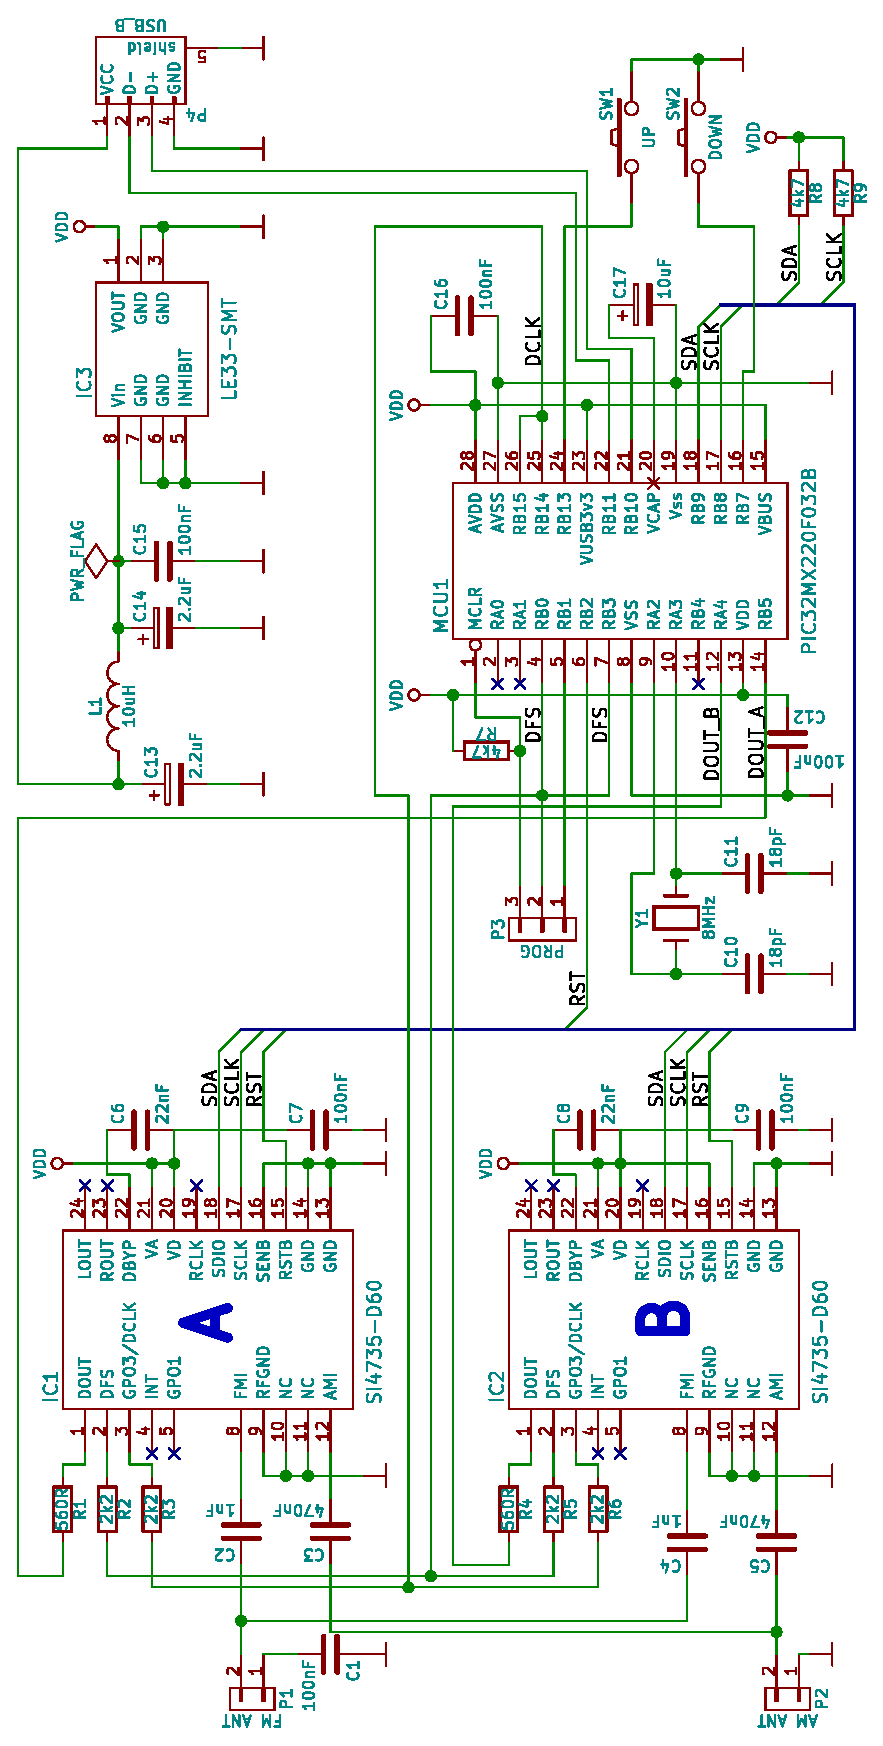
\includegraphics[scale=0.72]{figures/dfmt.eps}
\end{center}
 
\section{Rozpiska součástek}
\label{sec:ap-bom}
\begin{center}
\begin{tabular}{|l|r|r|r|l|}

\hline
Označení	& Název &	Počet	&	Pouzdro	&	Parametry\\
\hline
\makecell[l]{C1, C7, C9, C12,\\C15, C16}	&	Kondenzátor	&	6	&	1206	&	100 nF 5 \% X7R  50 V\\
\hline
C2, C4	&	Kondenzátor	&	2	&	1206	& 1 nF 5 \% X7R  50 V\\
\hline
C3, C5	&	Kondenzátor	&	2	&	1207	&	470 nF 5 \% X7R  50 V\\
\hline
C6, C8	&	Kondenzátor	&	2	&	1206	&	22 nF 5 \% X7R  50 V\\
\hline
C10, C11	&	Kondenzátor	&	2	&	1206	&	18 pF 5 \% X7R  50 V\\
\hline
C13, C14	&	Kondenzátor	&	2	&	B	&	2,2 $\mu$F 10 \% Tantal 16V \\
\hline
C17	&	Kondenzátor	&	1	&	B	&	10 $\mu$F 10 \% Tantal 16V \\
\hline
IC1, IC2	&	IO	&	2	&	SSOP24	&	SI4735-D60\\
\hline
IC3	&	IO	&	1	&	SO 8	&	LE33-SMT\\
\hline
L1	&	Tlumivka	&	1	&	1210	&	10 $\mu$H 10 \% 180 mA 1,6 $\Omega$\\
\hline
MCU1	&	IO	&	1	&	DIP28	&	PIC32MX220F032B\\
\hline
MCU1	&	Patice	&	1	&	DIP28	&	\\
\hline
P4	&	Konektor	&	1	&		&	USB B zásuvka  MOLEX 670688000 \\
\hline
R1, R4	&	Rezistor	&	2	&	1206	&	560 $\Omega$ 5 \%\\
\hline
R2, R3, R5, R6	&	Rezistor	&	4	&	1206	&	2,2 k$\Omega$ 5 \%\\
\hline
R7, R8, R9	&	Rezistor	&	3	&	1206	&	4,7 k$\Omega$ 5 \%\\
\hline
SW1, SW2	&	Tlačítko	&	2	&		&	TACT 613 N (neosazeno)\\
\hline
Y1	&	Krystal	&	1	&		&	8 MHz 30 ppm HC49SM 18 pF\\
\hline
-	&	Anténa &	1	&	& Vodič	38 cm AWG24\\
\hline

\end{tabular} 
\end{center}
%\end{landscape}

%\clearpage

%\InsertFigure{figures/Graf}{0.7\textwidth}{Nějaký graf}{fig:SampleGraph}

\section{Fotografie osazené desky plošných spojů}
\label{sec:ap-pcb}

\subsection*{Horní strana:}
\begin{center}
 \includegraphics[scale=1]{figures/pcb-top.jpg}
\end{center}

\subsection*{Spodní strana:}
\begin{center} 
 \includegraphics[scale=1]{figures/pcb-bot.jpg}
\end{center}


\end{document}
